% arara: pdflatex
%        File: ComplexAnalysis.tex
%     Created: Sat Jun 24 03:00 PM 2023 B
% Last Change: Sat Jun 24 03:00 PM 2023 B
%
\documentclass[a4paper, 12pt]{article}
\usepackage[]{amsmath}
\usepackage{amsthm}
\usepackage{amssymb}
\usepackage{mathtools}
\usepackage{soul}
\usepackage[]{graphicx}
\graphicspath{ {./images/} }
\usepackage{caption}
\usepackage{subcaption}

\theoremstyle{definition}
\newtheorem{definition}{Definition}
\newtheorem{exercise}{Exercise}
\newtheorem{example}{Example}
\newtheorem{remark}{Remark}

\numberwithin{definition}{section}
\numberwithin{exercise}{section}
\numberwithin{remark}{section}
\numberwithin{figure}{section}
\numberwithin{example}{section}

\newcommand{\R}{\mathbb{R}}
\newcommand{\C}{\mathbb{C}}

\title{Complex Analysis Summary}
\author{Paul Joo-Hyun Kim}
\begin{document}
\maketitle
\setcounter{section}{-1}
\section{Preface}
This note is for people studying complex analysis,
and got lost in the middle with bunch of technical explanations.
I wil try my best to be succinct as possible,
stating important results (mostly without proof, but a bit of justification).

\textbf{Warning}: This summary note is not a substitute for the lecture note.
Make sure you study from lecture note!

\section{Complex Plane and M\"obius Maps}
\subsection{Complex Plane and Complex Infinity}
We will be working in what's known as the \textit{extended complex plane}.
Define the symbol $\C_{\infty} \coloneqq \C \cup \left\{ \underbrace{\infty}_{\text{Complex Infinity}} \right\}$;
that is, I refer to the space of complex numbers
and infinity.

Note that in $\C_{\infty}$, $\infty$ is different from infinity in real numbers.
$\infty \coloneqq \frac{1}{0}$ is a value that is not ``larger'' or ``smaller'' than any number
(since we are talking about complex number\dots), but rather
a number on a complex plane at a really far distance from origin.

It is \textbf{WRONG} to say:
\begin{itemize}
    \item $\infty \geq a$ for any $a \in \C_{\infty}$
    \item $\infty \leq a$ for any $a \in \C_{\infty}$
\end{itemize}
However, it is \textbf{CORRECT}\footnote{
    Subtlety here: it seems a bit dodgy to say $\infty = \infty_{\infty}$,
    but this is matter of definition;
    you won't really encounter this type of ``philosophical'' problem
    in your exam.
} to say:
\begin{itemize}
    \item $|\infty| \geq |a|$ for any $a \in \C_{\infty}$.
\end{itemize}
$\infty$ is not like a point on $\C$, but rather like a gigantic circle that you can never reach.

\subsection{M\"obius Maps}
\begin{definition}[M\"obius Map]
    $\psi : \C_{\infty} \rightarrow \C_{\infty}$ is a \textbf{M\"obius map} if:
    \begin{equation*}
        \psi \left( z \right) \coloneqq \frac{az + b}{cz + d}
    \end{equation*}
    where $
    \begin{pmatrix}
        a & b \\ c & d
    \end{pmatrix}
    $ is a nonsingular matrix.
    (This restriction removes the possibility of $\frac{0}{0}$,
    or trivial maps (eg: Constant function).)

    One needs to be careful when defining this function at infinity,
    but it should be sensible.\footnote{
    That said, if you are supposed to define what a M\"obius map is,
    you are \textbf{required} to definitions involving infinity as well.
    }
\end{definition}
\begin{exercise}[Composition of two M\"obius map is a M\"obius map]
    Show that for two M\"obius maps $\psi_1, \psi_2$,
    its composition $\psi_1 \circ \psi_2$ is also a M\"obius map.
\end{exercise}
\begin{remark}
    Consider the $2 \times 2$-matrix-to-M\"obius-map map as follows:
    \begin{equation*}
        f (A) \coloneqq
        \begin{pmatrix}
            a_{11} & a_{12} \\ a_{21} & a_{22}
        \end{pmatrix}
        \mapsto
        \frac{a_{11} z + a_{12}}{a_{21} z + a_{22}}
    \end{equation*}
    Then it turns out that
    $f\left( AB \right) = f(A) f(B)$
\end{remark}
\begin{exercise}[Decomposition of M\"obius maps]
    It turns out that M\"obius maps can be written as composition of
    \begin{itemize}
        \item translation
        \item dialation (``scaling by nonzero constant'')
        \item inversion ($z \mapsto \frac{1}{z}$)
    \end{itemize}
    Prove this. (Hint: You can do a constructive proof.)
\end{exercise}
M\"obius maps also has a very convenient property:
\begin{exercise}[Circline to Circline]
    Show that M\"obius maps map circlines to circline.
    (This means a line will either map to a circle or a line,
    and also a circle will either map to a circle or a line.)

    (Note: This is a boring long tedious proof, that probably won't be asked in exam,
    but don't take my word for it.)
\end{exercise}

\section{Complex Differentiability}
Complex differentiability is one of the highlights of the complex analysis.
\begin{definition}[Differentiable Function AKA Holomorphic Function]
    Take $a \in \C$.
    Let $f:U \rightarrow \C$ be a function where $U$ is a neighbourhood\footnote{Some open set containing $a$.} of $a$.
    Then $f$ is \textbf{(complex) differentiable} or \textbf{holomorphic} at $a$ if
    \begin{equation*}
        f'(a) = \lim_{z \rightarrow a} \frac{f(z) - f(a)}{z - a}
    \end{equation*}
    exists, and call it derivative of $f$ at $a$.
    If $f$ is differentiable for all points in $U$, then it is said to be
    differentiable/holomorphic on $U$.
\end{definition}
\begin{remark}
    Note that the definition seems to be have trivially extended from real analysis.
    \ul{However, there is a subtlety}.
    The limit does not approach just from positive or negative side,
    but from any direction. (Figure \ref{fig: Real and Complex Limit})
    \begin{figure}[tbp]
        \centering
        \begin{subfigure}[b]{0.5\textwidth}
            \centering
            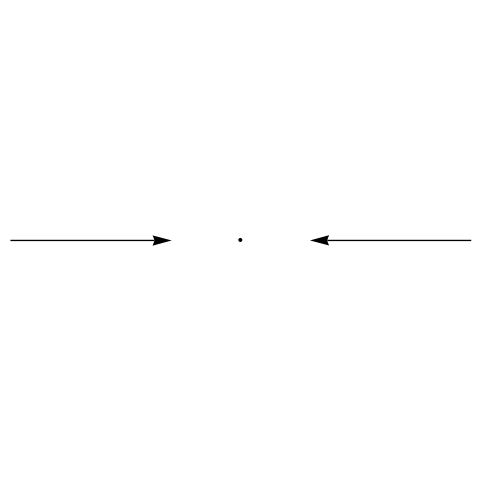
\includegraphics[width=\textwidth]{realLimit}
            \caption{Real Limit}
        \end{subfigure}
        \hfill
        \begin{subfigure}[b]{0.5\textwidth}
            \centering
            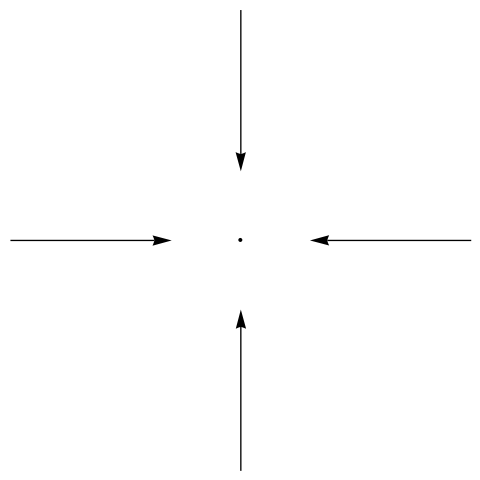
\includegraphics[width=\textwidth]{complexLimit}
            \caption{Complex Limit}
        \end{subfigure}
        \caption{Real limit (former) only concerns the approaching value from left and right side, but complex limit (latter) oncerns the approaching value from all direction.}
        \label{fig: Real and Complex Limit}
    \end{figure}
\end{remark}
\begin{exercise}[Differentiation Rules]
    Show that all differentiation rules from real analysis holds
    with holomorphic functions.
    \begin{itemize}
        \item Sum
        \item Product Rule
        \item Quotient Rule
        \item Chain Rule
    \end{itemize}
\end{exercise}
Due to the definition of complex limits being more restrictive,
a more nontrivial result follows.
\begin{exercise}[Cauchy-Riemann Equations]
    Let $a \in \C$ and $U$ be a neighbourhood of $a$.
    $f : U \rightarrow \C$ be holomorphic $a$.
    Write $f(z) = u(x,y) + i v(x,y)$ where $u,v$ are real functions
    and $z = x + iy$ where $x,y \in \R$.
    Then $\partial_x u, \partial_y u, \partial_x v, \partial_y v$ all exist,
    and the following \textbf{Cauchy-Riemann equations} hold:
    \begin{align*}
        \partial_x u &= \partial_y v \\
        \partial_x v &= - \partial_y u
    \end{align*}
(Hint: Figure \ref{fig: Real and Complex Limit} might give you an insight.)
\end{exercise}
\begin{remark}
    If Cauchy-Riemann does not hold, then it must mean that $f$ is not holomorphic! (Consider $f(z) = \bar{z}$. Cauchy-Riemann does not hold for any point, so it is nowhere holomorphic.)
\end{remark}
\begin{exercise}
    If $f(z) = u(x,y) + i v(x,y)$ is holomorphic on $U$,
    and $u,v$ are twice differentiable,
    deduce that $u$ and $v$ are \textit{harmonic}, that is,
    they satisfy the Laplace equation $\Delta u = \Delta v = 0$.
\end{exercise}
\begin{remark}
    It turns out complex plane reveals a lot about solving Laplace equation!
\end{remark}
Here is another kicker:
\begin{exercise}[Cauchy-Riemann to Holomorphic]
    If the partial derivatives exist and are continuously differentiable,
    Cauchy-Riemann implies holomorphicity.
\end{exercise}
\begin{remark}
    This means if you check that Cauchy-Riemann holds, you can immediately assume you can construct an analytic function!
\end{remark}
Holomorphic functions also have Taylor expansion:
\begin{remark}[Holomorphic functions have Taylor expansion]
    If $f$ is holormorphic at $a$, then
    in a neighbourhood of $a$, you can write
    \begin{equation*}
        f(z) = \sum_{n=0}^{\infty} c_n \left( z-a \right)^n
    \end{equation*}
    All the formulae for Taylor expansion holds (term-by-term differentiation, etc.)
\end{remark}
\begin{example}[Common Function Definitions]
    Here are definitions for some of the functions.
    \begin{align*}
        e^z = \exp z &\coloneqq \sum_{n=0}^{\infty} \frac{z^n}{n!} \\
        \cos{z} &\coloneqq \sum_{n=0}^{\infty} \left( -1 \right)^n \frac{z^{2n}}{\left( 2n \right)!} \\
        \cos{z} &\coloneqq \sum_{n=0}^{\infty} \left( -1 \right)^n \frac{z^{2n+1}}{\left( 2n + 1\right)!}
    \end{align*}
\end{example}
\begin{exercise}
    Show that
    \begin{align*}
        \cos{z} &= \frac{e^{iz} + e^{-iz}}{2} \\
        \sin{z} &= \frac{e^{iz} - e^{-iz}}{2i}
    \end{align*}
\end{exercise}
\begin{exercise}
    Show that $\exp \left( z+w \right) = \exp (z) \exp (w)$
\end{exercise}
\section{Branch Cut}
Sometimes, there is just no sensible way to define a function that it is holomorphic everywhere\dots
Two of the unfortunate (or fortunate) functions is the logarithm and square root.
We will first introduce the logarithm function.

Define logarithm function as:
\begin{equation*}
    \log z \coloneqq \log |z| + i \theta
\end{equation*}
where $\theta$ is the argument of $z$.

\begin{exercise}
    Verify that $\exp \left( \log z \right) = z$.
\end{exercise}

The choice of the interval for $\theta$ changes the behaviour of $\log z$ function.
For example, one could take the interval to be $\left[ 0, 2\pi \right)$,
or one could take it to be $\left[ - \pi, \pi \right)$,
or even just $\left[a, a + 2\pi\right)$ for some $a \in \R$.

The problem is that for given $z$, the argument of $z$ is not unique,
and if you try to define it continuously around a circle,
you will find that it is not possible\dots
(Figure \ref{fig: arg z multivalued}).
This means there needs to be some sort of contour from 0 that the function is not continuous on.
This is known as a \textbf{branch cut}, and you have total freedom to choose
based on what problem you want to solve.

\begin{figure}[tbp]
    \centering
    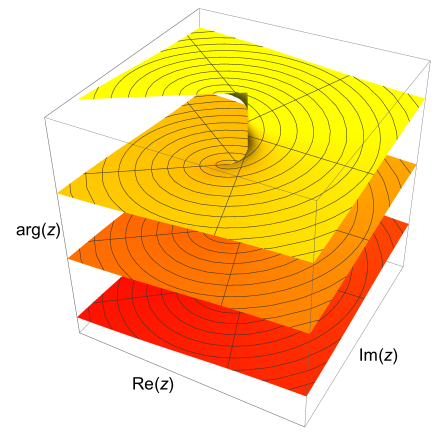
\includegraphics[scale=0.5]{argz}
    \caption{$\arg z$ being multivalued results in the need to introduce branch cut for logarithm.}
    \label{fig: arg z multivalued}
\end{figure}

\begin{example}[Where do we use branch cut?]
If you want to solve a problem with a fracture in an elastic solid (Figure \ref{fig: Crack Tip}),
one standard way to solve it is to find some holomorphic function outside of the crack $\left[ -c,c \right]$
satisfying some condition.
\begin{figure}[tbp]
    \centering
    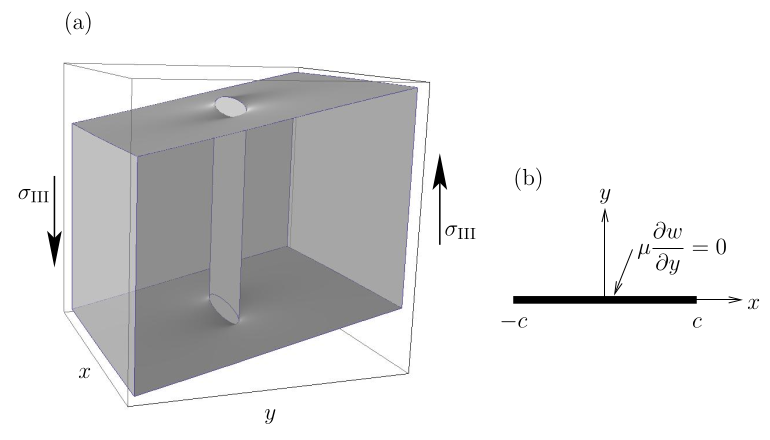
\includegraphics[scale=.5]{crackTip}
    \caption{Fracture in elastic material.}
    \label{fig: Crack Tip}
\end{figure}
It turns out that there is no function that is holomorphic everywhere satisfying that,
so you would define a ``branch cut'' to be the straight line $\left[ -c,c \right]$ to resolve it.
Then it is possible to define a function that is continuous away from the crack.
\end{example}

\begin{remark}
    When I say I am defining a branch cut,
    it means I am defining the function to be continuous away from the branch cut.
    \textbf{I am not the value of the function} at the function.
\end{remark}

Branch cuts are something that honestly makes more sense once you \textbf{played around with it for a while}.

\begin{example}[Logarithm: branch cut along positive real axis]
    See Figure \ref{fig: Log Positive Real} for the diagram of a branch cut along positive real axis.
    $\log z \coloneqq \log |z| + \theta i$ where $\theta \in \left[ 0, 2\pi \right)$ has a branch cut along positive real axis.
    Right above the positive real axis, $\theta$ takes the value 0, so $\left(\log x\right)_{+} = \log |x|$.
    On the other hand, right below the positive real axis, $\theta$ takes the value $2\pi$, so $\left( \log x \right)_{-} = \log |x| + 2\pi i$

    So you might ask: \textit{What is $\log z$ where $z \in \R^{>0}$?} and the answer is,
    you are asking the wrong question, because we can only define the ``limiting value'' on each side of the branch cut,
    NOT on the branch cut.
    \begin{figure}[tbp]
        \centering
        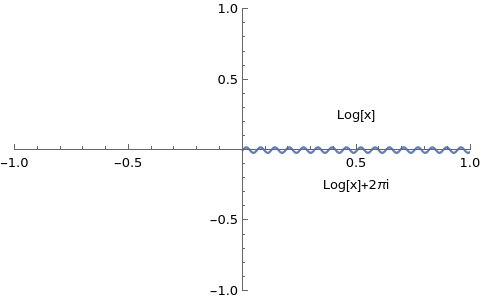
\includegraphics{logpositivereal}
        \caption{Logarithm function with branch cut along the positive real axis}
        \label{fig: Log Positive Real}
    \end{figure}
\end{example}
\begin{example}[Logarithm: branch cut along positive real axis]
    This time take $\theta \in \left[ -\pi, \pi \right)$.
    On the right side of the branch cut, we have $\theta = \pi$, so
    $\left( \log \left( yi \right) \right)_{+} = \log{y} + \pi i$,
    whereas on the left side, we have $\theta = -\pi$, so
    $\left( \log \left( yi \right) \right)_{-} = \log{y} - \pi$.

    \begin{figure}[tbp]
        \centering
        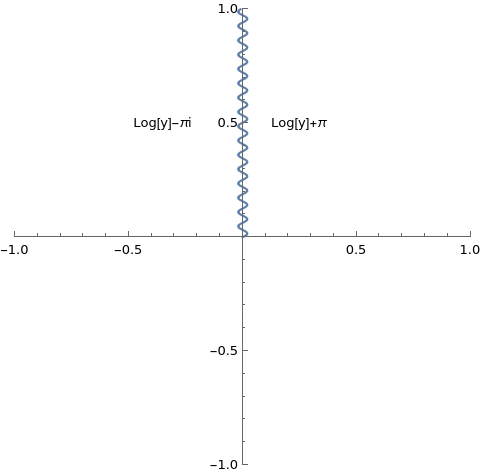
\includegraphics{logpositiveimaginary}
        \caption{Logarithm function with branch cut along the positive imaginary axis \textbf{Edit:} $\pi$ on the right side should be $\pi i$}
        \label{fig: Log Positive Imaginary}
    \end{figure}
\end{example}

\begin{exercise}[Square Root]
    Consider the definition of square root as given:
    \begin{equation*}
        z^{1/2} \coloneqq |z|^{1/2} e^{i \theta / 2}
    \end{equation*}
    (Note that I've just taken ``half'' as exponent in the polar form.)

    Define the branch cut along the negative real axis and evaluate $i^{1/2}$ in this branch.
    Define the branch cut along the negative imaginary axis and evaluate it again.
\end{exercise}
\begin{remark}
    In both square roots and logarithms, there was a point which the branch cut naturally starts from.
    These points are called \textbf{branch point};
    these are the points that you cannot avoid having a branch cut.
\end{remark}
\begin{remark}
    There is absolutely no need for a branch cut to be a straight line,
    and in some cases, it is more natural to define the branch cut in some other way (out of scope, however)
\end{remark}
\begin{exercise}
    Try defining some branch cuts of $\left( 1+z \right)^{1/2}$.
    What is the branch point in this case?
\end{exercise}
\begin{example}[Square Root Branch Cut of Elastic Crack]
    \label{eg: Square Root Branch Cut of Elastic Crack}
    Suppose you want to define the branch of the function $\left( z^2 - 1 \right)^{1/2}$
    such that it is holomorphic away from the branch cut $\left[ -1,1 \right]$.

    Consider writing the function in a following way:
    \begin{equation*}
        \left( z^2 - 1 \right)^{1/2} = \left( z-1 \right)^{1/2} \left( z+1 \right)^{1/2}
    \end{equation*}
    Now note that $\left( z-1 \right)^{1/2}$ and $\left( z+1 \right)^{1/2}$ need branch cuts.
    One way to define them is through:
    \begin{align*}
        \left( z-1 \right)^{1/2} &= r_1^{1/2} e^{i\theta_1 / 2} \\
        \left( z+1 \right)^{1/2} &= r_2^{1/2} e^{i\theta_2 / 2}
    \end{align*}
    where $\theta_1, \theta_2 \in \left[ -\pi, \pi \right)$ (See Figure \ref{fig: Crack Tip 2}\footnote{
            The angle range is not a mistake, even though it might seem a bit unintuitive.
    })
    \begin{figure}[tbp]
        \centering
        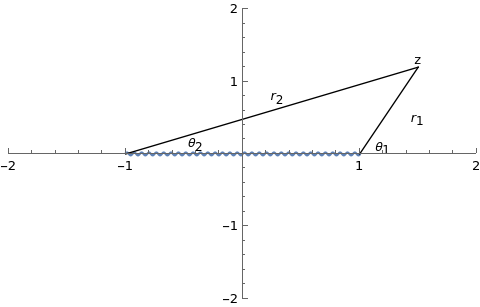
\includegraphics{crackTip2}
        \caption{$r_1, r_2, \theta_1, \theta_2$ as shown. The point on the upper right is the $z$.}
        \label{fig: Crack Tip 2}
    \end{figure}
    Hence, we get our branch cut between -1 and 1:
    \begin{equation*}
        \left( z^2 - 1 \right)^{1/2} = r_1^{1/2} r_2^{1/2} e^{i \left( \frac{\theta_1 + \theta_2}{2} \right)}
    \end{equation*}
\end{example}
\begin{exercise}
    Show that the branch cut defined on Example \ref{eg: Square Root Branch Cut of Elastic Crack}
    has different limiting values across the branch cut.
    \textbf{Again, the angle range given is not a mistake!}
\end{exercise}

\end{document}


